%@@@@@@@@@@@@@@@@@@@@@@@@@@@@@@@@@@@@@@@@@@@@@@@@@@
\chapter{Tracking in quantized videos}
\label{chap_TRK_quantized}	
%@@@@@@@@@@@@@@@@@@@@@@@@@@@@@@@@@@@@@@@@@@@@@@@@@@

%#######################
\section{Region tracking}
%#######################
\begin{figure}[t]
	\center
	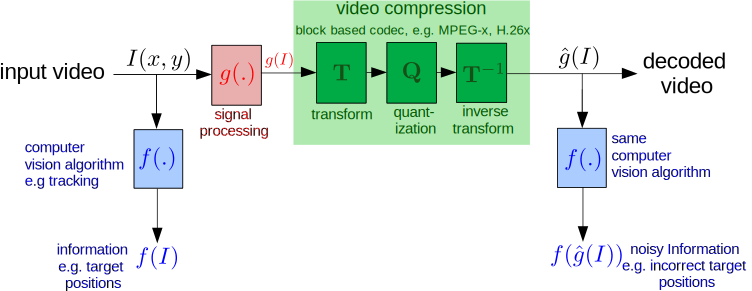
\includegraphics[width=1.0\textwidth]{figs/ICIP2009_SolutionThroughSigProc.pdf}
	\caption{Visual tracking, overview}
\end{figure}


\begin{figure}[t]
	\center
	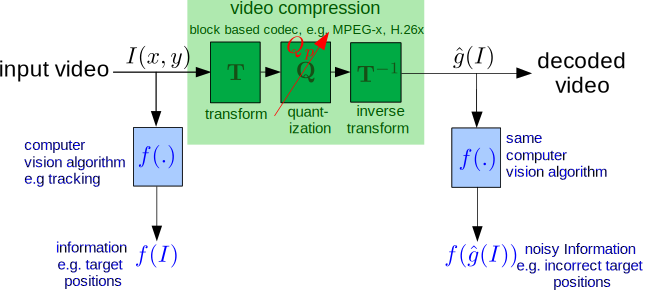
\includegraphics[width=1.0\textwidth]{figs/TRK_IPCV2009_BlockDiagram_2_VarPar_2.pdf}
	\caption{Visual tracking, overview}
\end{figure}

\begin{figure}[t]
	\center
	\includegraphics[width=1.0\textwidth]{figs/ICIP2009_PETS2001_FN_00592_snapshotVVG.pdf}
	\caption{Visual tracking, overview}
\end{figure}

	\begin{figure}
		\centering
		\subfigure[Ground truth]
			{
				\includegraphics[width=.45\textwidth]{figs/TRK_IPCV2009_PETS2001_FN_00592_outputGroundTruth}
				\label{fig:PETS2001_Frame592_Ground}
			}
		\subfigure[Base]
			{
				\includegraphics[width=.45\textwidth]{figs/TRK_IPCV2009_PETS2001_FN_00592_outputBaseline}
				\label{fig:PETS2001_Frame592_Base}
			}
		\subfigure[SigProc]
			{
				\includegraphics[width=.45\textwidth]{figs/TRK_IPCV2009_PETS2001_FN_00592_outputSigProc}
				\label{fig:PETS2001_Frame592_SigProc}
			}
		\subfigure[VarPar]
			{
				\includegraphics[width=.45\textwidth]{figs/TRK_IPCV2009_PETS2001_FN_00592_outputVarPar}
				\label{fig:PETS2001_Frame592_VarPar}
			}	
	\end{figure}


	\begin{figure}
		\includegraphics[width=1.0\textwidth]{figs/ICIP2009_PETS2007_FN_00340_snapshotVVG.pdf}
	\end{figure}


	\begin{figure}%[htp]
		\centering
		\subfigure[Ground truth]
			{
				\includegraphics[width=.45\textwidth]{figs/TRK_IPCV2009_PETS2007_FN_00340_outputGroundTruth}
				\label{fig:PETS2007_Frame340_Ground}
			}
		\subfigure[Base]
			{
				\includegraphics[width=.45\textwidth]{figs/TRK_IPCV2009_PETS2007_FN_00340_outputBaseline}
				\label{fig:PETS2007_Frame340_Base}
			}
		\subfigure[SigProc]
			{
				\includegraphics[width=.45\textwidth]{figs/TRK_IPCV2009_PETS2007_FN_00340_outputSigProc}
				\label{fig:PETS2007_Frame340_SigProc}
			}
		\subfigure[VarPar]
			{
				\includegraphics[width=.45\textwidth]{figs/TRK_IPCV2009_PETS2007_FN_00340_outputVarPar}
				\label{fig:PETS2007_Frame340_VarPar}
			}	
	\end{figure}


	\begin{table}
		\centering
		\begin{tabular}{|l|c|c|c|c|}
			\hline
			\multicolumn{5}{|c|}{Accuracy (distance from ground truth)} \\
			\hline
			Dataset & Qp & Baseline & $SigProc$  & $VarPar$\\ 
			\hline
			\multirow{4}{*}{PETS2001} 
				&5  & 8.7 	&   2.4 &   2.1 \\
				&16 & 75.4 &  10.3 &   2.1\\
				&27 &16.0 	&  12.7 &   2.1\\
				&31 &13.7 &  10.2 &   2.1\\
			\hline
			\multirow{3}{*}{PETS2007} 
				&5 &5.8 &   3.5 &   1.0\\
				&16 &85.1 &   4.2 &   1.0\\
				&27 &71.8 &   3.5 &   1.0\\
				&31 &15.2 &  35.8 &   1.0\\
			\hline
			\multirow{1}{*}{Average}
			& - & 36.5 & 10.3 & 1.6 \\  
			\hline
		\end{tabular}
	\end{table}

%#######################
\section{Contour tracking}
%#######################
	\begin{figure}
		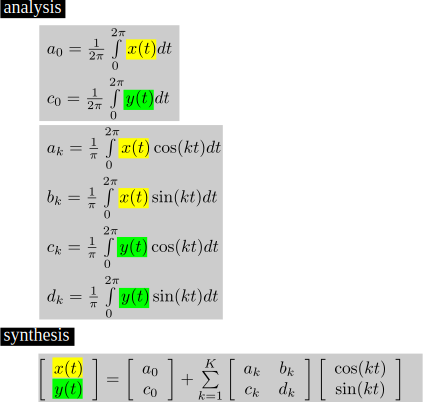
\includegraphics[height=0.8\textheight]{figs/theory_curves_ellipticalFourier.pdf}
	\end{figure}

		\begin{figure}
			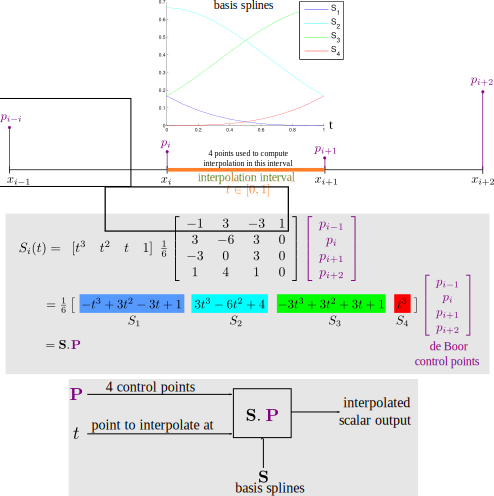
\includegraphics[height=0.85\textheight]{figs/theory_curves_UniformCubicBsplines.pdf}
		\end{figure}
